\documentclass[12pt]{extarticle}
%Some packages I commonly use.
\usepackage[english]{babel}
\usepackage{graphicx}
\usepackage{framed}
\usepackage{cancel}
\usepackage[normalem]{ulem}
\usepackage{amsmath, amsthm, amssymb, amsfonts}
\usepackage{enumerate}
\usepackage[utf8]{inputenc}
\usepackage[top=1 in,bottom=1in, left=1 in, right=1 in]{geometry}

\title{MECH511 Assignment 1 Multigrid}
\author{Nick Earle}
\date{February 4, 2019}

\begin{document}

\maketitle

\section{Mesh-to-Mesh Transfer Operators}

\begin{enumerate}[(a)]
    \item Fine-to-coarse
    
        Similar to the one-dimensional case, each cell, which is the culmination of four cells will simply equal the average of those four cells:
        \begin{equation*}
            I_{h\rightarrow H}: \qquad e^H_{i,j} = \frac{e^h_{2i-1,2j}+e^h_{2i-1,2j-1}+e^h_{2i,2j}+e^h_{2i,2j-1}}{4}
        \end{equation*}
        
    \item Coarse-to-fine by Injection
    
        As with the 1D case, each cell within the larger cell, will retain that same value:
        \begin{equation*}
            I_{H\rightarrow h}: \qquad e^h_{2i-1,2j} = e^h_{2i-1,2j-1} = e^h_{2i,2j} = e^h_{2i,2j-1} = e^H_{i,j}
        \end{equation*}
        
    \item Coarse-to-fine by Interpolation
        
        Using bi-linear interpolation for each cell, that is the same interpolation as the 1d case for all of the adjacent cells in both directions, we can then sum each fraction to get the amount of each of the coarse cells to use. We get the following weights:
        \begin{equation*}
            \renewcommand{\arraystretch}{2}
            \left[ \begin{array}{c | c | c}
            \frac{1}{4} & \frac{1}{2} & \frac{1}{4} \\
            \hline
            \frac{1}{4} & \frac{1}{2} & \frac{1}{4} \\
            \hline
            \frac{1}{4} & \frac{1}{2} & \frac{1}{4}
            \end{array} \right]
            \times
            \renewcommand{\arraystretch}{2}
            \left[ \begin{array}{c|c|c}
            \frac{1}{4} & \frac{1}{4} & \frac{1}{4} \\
            \hline
            \frac{1}{2} & \frac{1}{2} & \frac{1}{2} \\
            \hline
            \frac{1}{4} & \frac{1}{4} & \frac{1}{4}
            \end{array} \right]
            =
            \renewcommand{\arraystretch}{2}
            \left[ \begin{array}{c|c|c}
            \frac{1}{16} & \frac{1}{8} & \frac{1}{16} \\
            \hline
            \frac{1}{8} & \frac{1}{4} & \frac{1}{8} \\
            \hline
            \frac{1}{16} & \frac{1}{8} & \frac{1}{16}
            \end{array} \right]
        \end{equation*}
        Applying these weights to the coarse mesh we get the following equations for each fine cell:
        \begin{equation*}
            e^h_{2i-1,2j} = \frac{9}{16}e^H_{i,j} + \frac{3}{16}e^H_{i-1,j} + \frac{3}{16}e^H_{i,j+1} + \frac{1}{16}e^H_{i-1,j+1}
        \end{equation*}
        \begin{equation*}
            e^h_{2i-1,2j-1} = \frac{9}{16}e^H_{i,j} + \frac{3}{16}e^H_{i-1,j} + \frac{3}{16}e^H_{i,j-1} + \frac{1}{16}e^H_{i-1,j-1}
        \end{equation*}
        \begin{equation*}
            e^h_{2i,2j} = \frac{9}{16}e^H_{i,j} + \frac{3}{16}e^H_{i+1,j} + \frac{3}{16}e^H_{i,j+1} + \frac{1}{16}e^H_{i+1,j+1}
        \end{equation*}
        \begin{equation*}
            e^h_{2i,2j-1} = \frac{9}{16}e^H_{i,j} + \frac{3}{16}e^H_{i+1,j} + \frac{3}{16}e^H_{i,j-1} + \frac{1}{16}e^H_{i+1,j-1}
        \end{equation*}
\end{enumerate}

\newpage
\section{Amplification Factor}

    Given the Point Jacobi scheme below, on the domain $x \in [0,1]$
    \[ T^{n+1}_i = T^n_i + \omega\left(\frac{T^n_{i+1}+T^n_{i-1}}{2}-T^n_i\right)\]
    \begin{enumerate}[(a)]
        \item Amplification factor, using $T_i = \exp(Iik\pi\Delta x)$
        \begin{equation*}
        \begin{split}
            T^{n+1}_i & = T^n_i + \frac{\omega}{2}T^n_{i+1} +\frac{\omega}{2}T^n_{i-1} - T^n_i \\
            & = \exp(Iik\pi\Delta x) + \frac{\omega}{2}\exp(I(i+1)k\pi\Delta x) + \frac{\omega}{2}\exp(I(i-1)k\pi\Delta x) - \omega\exp(Iik\pi\Delta x) \\
            & = \exp(Iik\pi\Delta x)\left(1 + \frac{\omega}{2}\exp(Ik\pi\Delta x) + \frac{\omega}{2}\exp(-Ik\pi\Delta x) -\omega\right)
        \end{split}
        \end{equation*}
        \bigskip
        \begin{equation*}
        \begin{split}
            \frac{T^{n+1}_i}{T^n_i} & = 1 - \omega + \frac{\omega}{2}\left(\exp{Ik\pi\Delta x} + \exp{-Ik\pi\Delta x}\right) \\
            & = 1 - \omega + \frac{\omega}{\cancel{2}}\left( \cos{k\pi\Delta x} + \cancel{I\sin{k\pi\Delta x}} + \cos{k\pi\Delta x} - \cancel{I\sin{k\pi\Delta x}}\right)\\
            & = 1 - \omega\left(1 - \cos{k\pi\Delta x}\right)
        \end{split}
        \end{equation*}
        
        \item No local maximum in high-frequency range
        
        The following plots all use $i_{max}=100$, while the plot below shows that there is indeed no local maximum in the high-frequency range of the amplification factor $k \ge i_{max}/2$
        \begin{figure}[h]
            \centering
            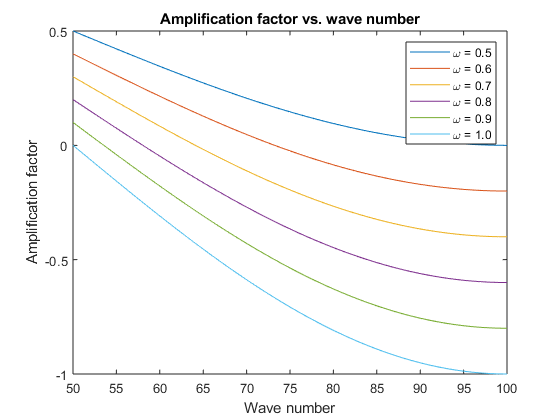
\includegraphics[scale = 0.7]{singlepass_amp}
        \end{figure}
        
        \newpage
        \item $\omega$ that minimizes maximum $\sigma$
        
        Matlab's \emph{fminsearch} function was used to find the over-relaxation constant that minimizes the maximum value of the amplification factor, which was found to be true true when the absolute value at $k = i_{max}/2$ equals that of $k = i_{max}$.
        \vspace{-2mm}
        \[ \omega_{opt} = 0.6667\]
        \[ \sigma_{opt} = 0.3334\]
        \begin{figure}[h]
        \vspace{-10mm}
            \centering
            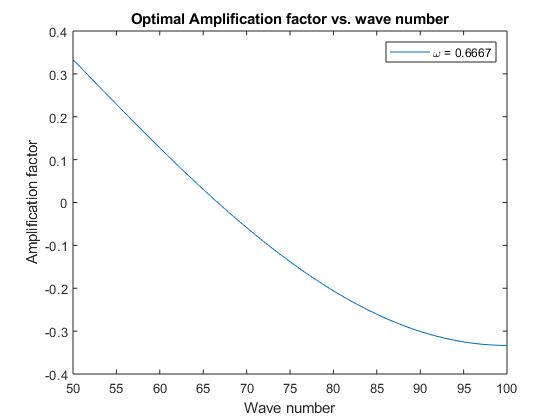
\includegraphics[scale = 0.7]{singlepass_amp_opt.png}
        \vspace{-5mm}
        \end{figure}
        
        The optimum $\omega$ for this scheme is different than that of the single-mesh scheme because here we are trying the minimize the high-frequency error as opposed to the low-frequency error achieved when $\omega > 1$.
        
        \item Two passes
        
        For two passes where the amplification factor equals the product of that of the two single passes, there does exist a local minimum in the high-frequency range, shown here using $\omega_1 = 0.6$ and $\omega_2 = 0.8$.
        
        \begin{figure}[ht]
            \centering
            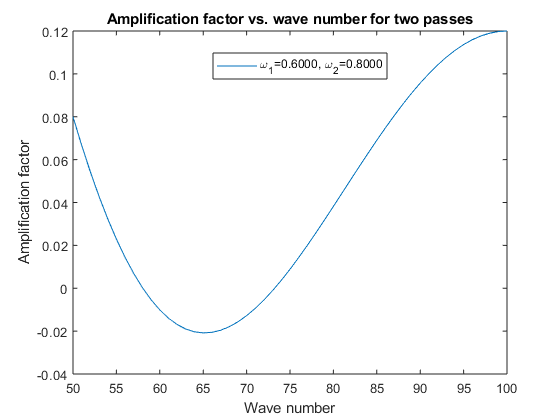
\includegraphics[scale = 0.7]{doublepass_amp.png}
        \end{figure}
        
        \newpage
        \item Optimal $\omega_1$ and $\omega_2$ for two-pass case
        
        As with the single pass case, the optimal over-relaxation factors are when the amplification factors of $k = i_{max}/2$ equals that of $k = i_{max}$, from here we can simplify the amplification factor to find the relation of over-relaxation factors that achieve this result.
        \vspace{-3mm}
        \begin{equation*}
            \sigma = (1 - \omega_1(1-\cos{k\pi\Delta x})) (1 - \omega_2(1-\cos{k\pi\Delta x}))
        \end{equation*}
        Equating this at each end, remembering $\Delta x = 1/i_{max}$ we get:
        \begin{align*}
            (1 - \omega_1(1-\cos(\pi/2)))(1 - \omega_2(1-\cos(\pi/2))) &= (1 - \omega_1(1-\cos{\pi}))(1 - \omega_2(1-\cos{\pi})) \\
            (1 - \omega_1) (1 - \omega_2) &= (1 - 2\omega_1) (1 - 2\omega_2) \\
            1 - \omega_1 - \omega_2 + \omega_1\omega_2 &= 1 - 2\omega_1 - 2\omega_2 + 4\omega_1\omega_2 \\
            \omega_1 + \omega_2 - 3\omega_1\omega_2 &= 0 \\
            \omega_1 &= \frac{\omega_2}{3\omega_2-1}
        \end{align*}
        
        Using this relation and knowing that the minimum value is equal and opposite sign to the maximum we can perform a similar search as above using \emph{fminsearch} to find the optimal $\omega_1$ and $\omega_2$ which are:
        \begin{align*}
            \omega_{1opt} &= 0.5395 \\
            \omega_{2opt} &= 0.8724 \\
            \sigma_{opt} &= 0.0588
        \end{align*}
        
        This results in an amplification factor almost six times smaller than the single pass case.
        
        \begin{figure}[h]
            \centering
            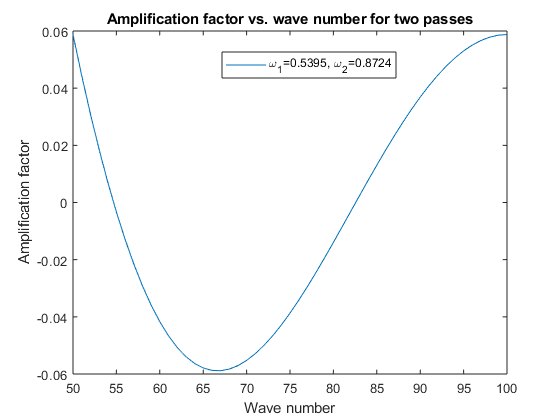
\includegraphics[scale = 0.7]{doublepass_amp_opt.png}
        \end{figure}
        
        \newpage
        \item Single pass vs. double pass
        
        Comparing the optimal single squared and double pass cases:
        
        \begin{figure}[h]
            \centering
            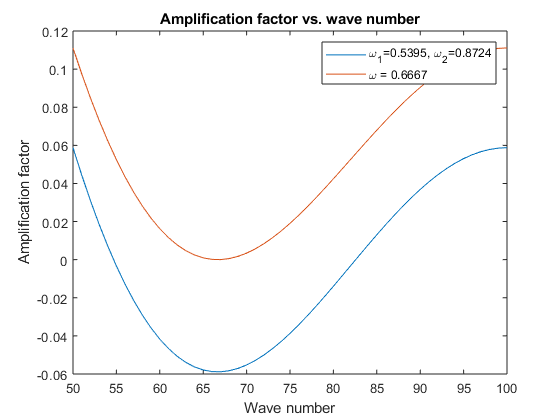
\includegraphics[scale = 0.7]{single_sqr_double.png}
        \end{figure}
        
    \end{enumerate}

\end{document}
